\chapter{Cinématique II: Le mouvement}
\label{sec:cinediff}



%%%%%%%%%%%%%%%%%%%%%%%%%%%%%%%%%%%%%%%%%%%%%%%%%%%%%%%%%%%%%%%%%%%%%%%%%%%%%%%%%%%%%%%%%%%%%%%%%%%%%%%%%%%%%%%%%%%%%%%%%%%%%%%%%%%%%%%%%%%%
\section{Cinématique différentielle des robots manipulateurs}
%%%%%%%%%%%%%%%%%%%%%%%%%%%%%%%%%%%%%%%%%%%%%%%%%%%%%%%%%%%%%%%%%%%%%%%%%%%%%%%%%%%%%%%%%%%%%%%%%%%%%%%%%%%%%%%%%%%%%%%%%%%%%%%%%%%%%%%%%%%%


La cinématique différentielle c'est l'étude de la relation entre le mouvement des joints et le mouvement associé de l'effecteur. Dans le chapitre \ref{sec:cine1}, les fonctions reliant la position de l'effecteur $\col{r}$ et la configuration du robot dans l'espace des joints $\col{q}$ ont été étudiées:
%%%%%%%%%%%%%%%%
\begin{equation}
\text{Cinématique directe:}  \quad \col{r} = f\left( \, \col{q} \, \right)  \quad  \text{inverse:} \quad \col{q} = f^{-1}\left( \, \col{r}  \, \right) 
\end{equation}
%%%%%%%%%%%%%%%

Plusieurs méthodes en robotique sont plutôt basées sur les fonctions qui relient la vitesse de l'effecteur $\col{\dot{r}}$ à la vitesse des joints $\col{\dot{q}}$. Ces fonctions prennent la forme suivante:
%%%%%%%%%%%%%%%%
\begin{equation}
\text{Cinématique différentielle directe:} \quad \col{\dot{r}} = J\left( \, \col{q} \, \right) \, \col{\dot{q}}   \quad \text{inverse:} \quad \col{\dot{q}} = J^{-1}\left( \, \col{q} \, \right) \, \col{\dot{r}}
\end{equation}
%%%%%%%%%%%%%%%
Les fonctions de cinématique différentielle implique une matrice Jacobienne qui relit des déplacements infinitésimales des joints aux déplacements infinitésimales de l'effecteur:
%%%%%%%%%%%%%%%%
\begin{equation}
\text{Matrice Jacobienne:} \quad J\left( \col{q} \right) = \frac{\partial \col{r}}{\partial \col{q}}
\end{equation}
%%%%%%%%%%%%%%%%
La composante $J_{ij}$ de la matrice correspond à la variation de la coordonnée $r_i$ de l'effecteur, due à un déplacement unitaire du joint $q_j$. D'un point de vue mathématique, la matrice Jacobienne $J$ correspond au gradient de la fonction multi-variable $\col{r} = f\left( \, \col{q} \, \right)$. Ensuite, la relation qui relit les vitesses est relié à la relation entre les déplacements infinitésimals par le principe des dérivées en chaînes:
%%%%%%%%%%%%%%%%
\begin{equation}
\text{Dérivées en chaînes:} \frac{d \col{r}}{dt} = \left( \frac{\partial \col{r}}{\partial \col{q}} \right) \frac{d \col{q}}{dt} 
\end{equation}
%%%%%%%%%%%%%%%%

%%%%%%%%%%%%%%%%%%%%%%%%%%%%%%%%%%%%%%%%%%%%%%%%%%%%%%%%%%%%%%%%%%%%%%%%%%%%%%%%%%%%%%%%%%%%%%%%%%%%%%%%%%%%%%%%%%%%%%%%%%%%%%%%%%%%%%%%%%%%
\subsection{La matrice Jacobienne}
%%%%%%%%%%%%%%%%%%%%%%%%%%%%%%%%%%%%%%%%%%%%%%%%%%%%%%%%%%%%%%%%%%%%%%%%%%%%%%%%%%%%%%%%%%%%%%%%%%%%%%%%%%%%%%%%%%%%%%%%%%%%%%%%%%%%%%%%%%%%

\paragraph{Unités} Typiquement pour les analyse de cinématique différentielle, les variables de sortie sont les DDL de translation de l'effecteur, la pose complète de l'effecteur ou bien des variables qui décrivent les DDL de l'espace de la tâche; et les variables d'entrée sont les vitesse angulaire des joints du robot. Les unités des composantes $J_{ij}$ de la matrice Jacobienne associée sont donc typiquement soit des unités de distance qui correspondent à des \textit{bras de levier}, ou bien des ratios adimensionnels de vitesses angulaires. 

\paragraph{Non-linéarité} Il est important de noté que généralement la matrice Jacobienne est une fonction de la configuration $\col{q}$ du robot. Comme la fonction de cinématique directe est généralement hautement non-linéaire, l'effet d'un déplacement infinitésimal d'un joint sur l'effecteur dépend considérablement de la configuration initiale. 

\paragraph{Colonnes} Comme illustré à la Figure \ref{fig:jaco_graph}, dans le contexte de cinématique différentiel, la colonne $j$ de la matrice Jacobienne correspond à un vecteur déplacement de l'effecteur due au mouvement du joint $j$. 

%%%%%%%%%%%%%%%%%%%%%%%%%%%%%%%%%%%%%%%%%%%%%%%%%%
%\begin{figure}[H]
	%\centering
		%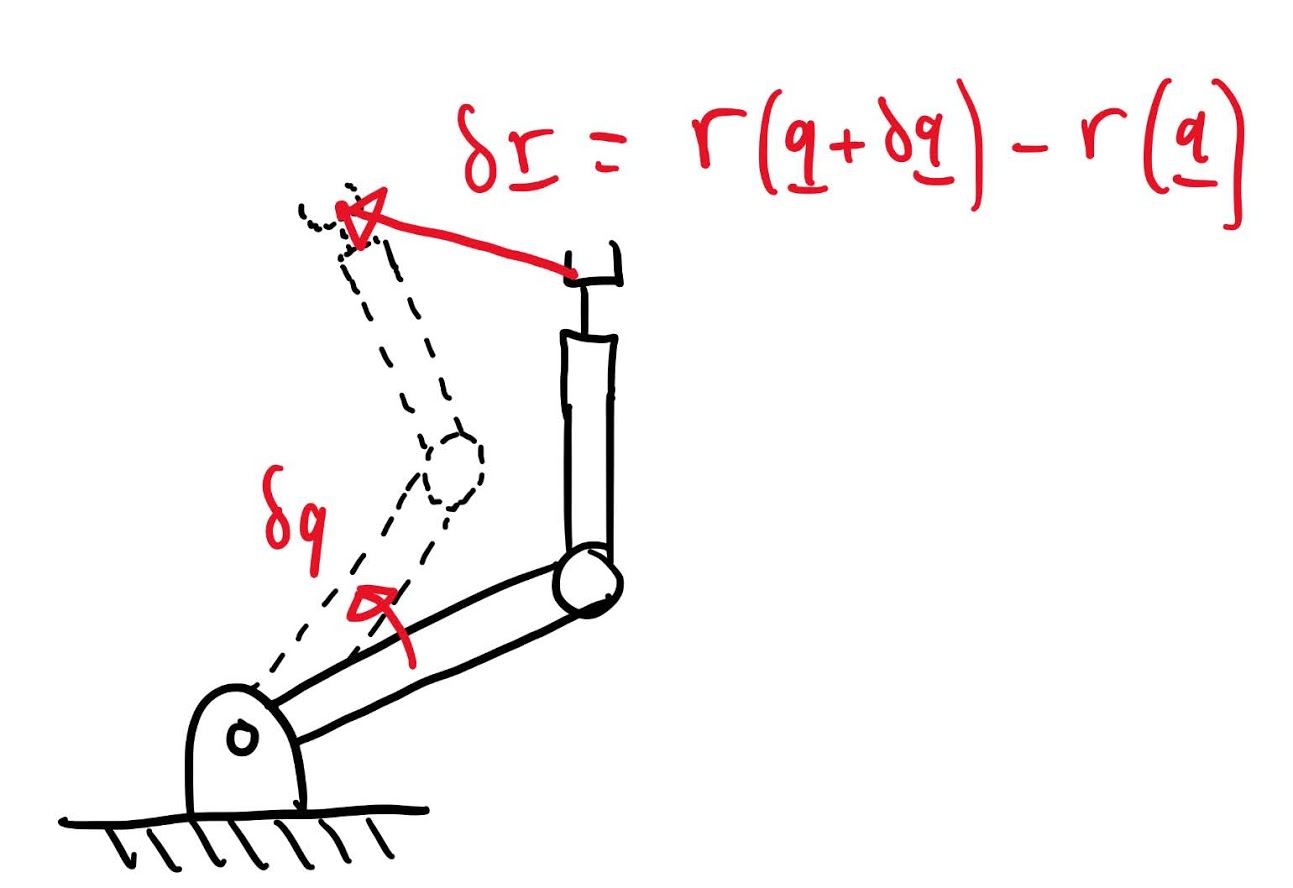
\includegraphics[width=0.75\textwidth]{diff_kin.jpg}
	%\caption{Cinématique différentielle}
	%\label{fig:diff_kin}
%\end{figure}
%%%%%%%%%%%%%%%%%%%%%%%%%%%%%%%%%%%%%%%%%%%%%%%%%%


%%%%%%%%%%%%%%%%%%%%%%%%%%%%%%%%%%%%%%%%%%%%%%%%%
\begin{figure}[H]
\vspace{-5pt}
	\centering
		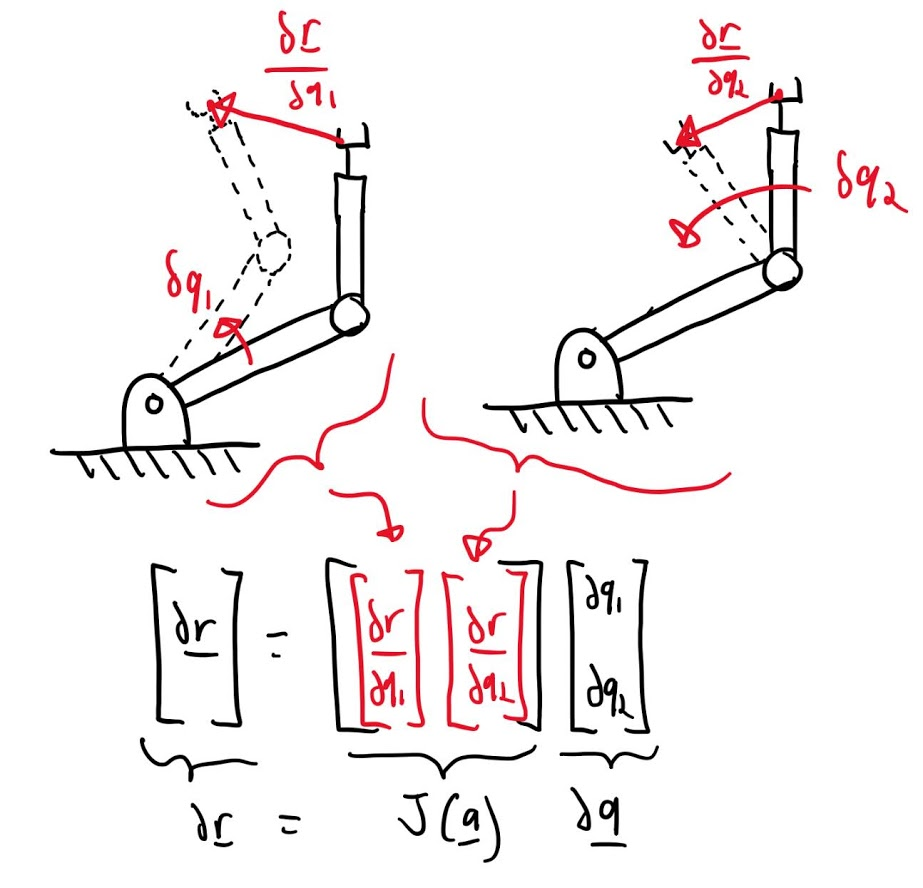
\includegraphics[width=0.55\textwidth]{jaco_graph.jpg}
	\caption{Illustration vectorielle du Jacobian du manipulateur}
	\vspace{-5pt}
	\label{fig:jaco_graph}
\end{figure}
%%%%%%%%%%%%%%%%%%%%%%%%%%%%%%%%%%%%%%%%%%%%%%%%%



%%%%%%%%%%%%%%%%%%%%%%%%%%%%%%%%%%%%%%%%%%%%%%%%%%%%%%%%%%%%%%%%%%%%%%%%%%%%%%%%%%%%%%%%%%%%%%%%%%%%%%%%%
\subsection{Exemples de cinématique différentielle pour des robots manipulateurs}

%%%%%%%%%%%%%%%%%%%%%%%%%%%%%%%%%%%%%%%%%%%%%%%%%%%%%%%%%%%%%%%%%%%%%%%%%%%%%%%%%%%%%%%%%%%%%%%%%%%%%%%%%
\subsubsection{Cinématique différentielle d'un robot cartésien}

La Figure \ref{fig:jaco_robot_cart} illustre un robot planaire constitué de deux actionneurs linéaires basé sur des vis à billes qui sont assemblés à 90 degrées. 
%%%%%%%%%%%%%%%%%%%%%%%%%%%%%%%%%%%%%%%%%%%%%%%%%
\begin{figure}[H]
	\vspace{-5pt}
	\centering
		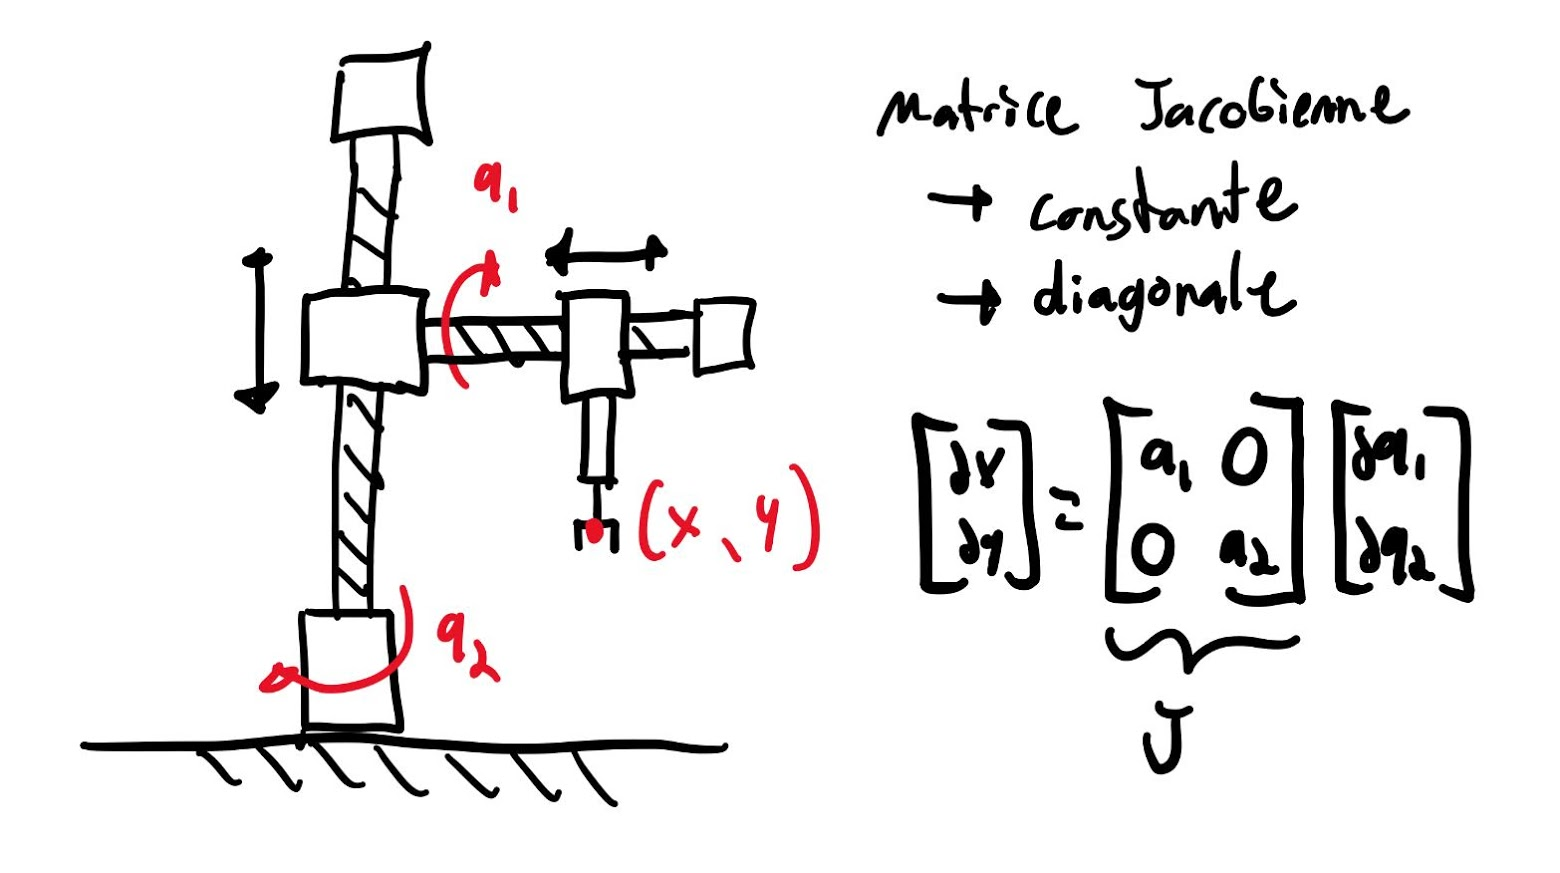
\includegraphics[width=0.65\textwidth]{jaco_robot_cart.jpg}
	\caption{Jacobien pour un robot cartésien}
	\vspace{-5pt}
	\label{fig:jaco_robot_cart}
\end{figure}
%%%%%%%%%%%%%%%%%%%%%%%%%%%%%%%%%%%%%%%%%%%%%%%%%

Pour ce robot, chaque actionneur linéaire contrôle de façon indépendante la translation $x$ et $y$ de l'effecteur, la fonction de cinématique directe est donnée par :
%%%%%%%%%%%%%%%%
\begin{align}
\quad \col{r} &= f\left( \, \col{q} \, \right)  \\
\left[ \begin{array}{c} x \\ y  \end{array} \right]  &= \left[ \begin{array}{c} a_1 q_1 \\ a_2 q_2  \end{array} \right]
\label{eq:fwdkinlin}
\end{align}
%%%%%%%%%%%%%%%
ou les variables $a_i$ sont des constantes qui relient la rotation angulaire des vis aux déplacements linéaires. La relation différentielle peut alors être calculée:
%%%%%%%%%%%%%%%%%%%%%%%%%%%%%%%%%%%
\begin{align}
\underbrace{ \left[ \begin{array}{c} \dot{x} \\ \dot{y}  \end{array} \right] }_{\dot{\col{r}}}
 &= 
\underbrace{ \left[ \begin{array}{c c } 
\frac{\partial x }{\partial q_1}   & \frac{\partial x }{\partial q_2} \\ 
\frac{\partial y }{\partial q_1}   & \frac{\partial y }{\partial q_2}
\end{array} \right]  }_{ J } 
\underbrace{ \left[ \begin{array}{c} 
\dot{q}_1 \\ 
\dot{q}_2 
\end{array} \right]}_{ \dot{\col{q}} } \\
%%%%%%%%%%%%%
\underbrace{ \left[ \begin{array}{c} \dot{x} \\ \dot{y}  \end{array} \right] }_{\dot{\col{r}}}
 &= 
\underbrace{ \left[ \begin{array}{c c } 
a_1 & 0 \\ 
0   & a_2
\end{array} \right]  }_{ J } 
\underbrace{ \left[ \begin{array}{c} 
\dot{q}_1 \\ 
\dot{q}_2 
\end{array} \right]}_{ \dot{\col{q}} } \\
\end{align} 
%%%%%%%%%%%%%%%%%%%%%%%%%%%%%%%%%%%

Il est a noter ici que: \textbf{1)} la matrice Jacobienne est diagonale car chaque joint influence indépendamment un seul DDL de l'effecteur. \textbf{2)} la matrice Jacobienne est constante et indépendante de $\col{q}$ car la relation de cinématique directe (\eqref{eq:fwdkinlin}) est linéaire. 


%%%%%%%%%%%%%%%%%%%%%%%%%%%%%%%%%%%%%%%%%%%%%%%%%%%%%%%%%%%%%%%%%%%%%%%%%%%%%%%%%%%%%%%%%%%%%%%%%%%%%%%%%
\subsubsection{Cinématique différentielle d'un robot à deux joints}

%%%%%%%%%%%%%%%%%%%%%%%%%%%%%%%%%%%%%%%%%%%%%%%%%
\begin{figure}[H]
	\centering
		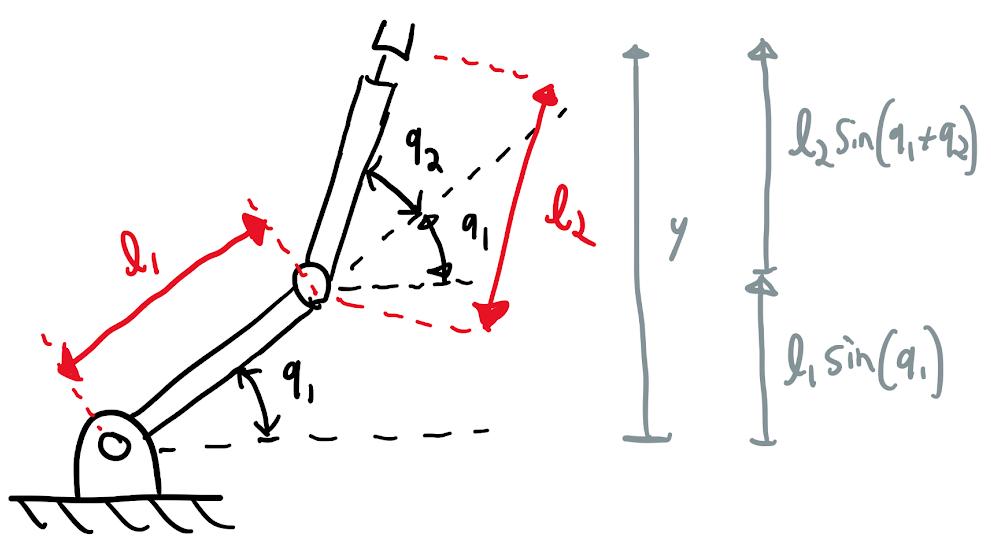
\includegraphics[width=0.65\textwidth]{robot_2dof.png}
	\caption{Robot à deux joints}
	\label{fig:robot_2dof}
\end{figure}
%%%%%%%%%%%%%%%%%%%%%%%%%%%%%%%%%%%%%%%%%%%%%%%%%

Pour un robot manipulateur planaire à deux DDL, comme illustré à la Figure \ref{fig:robot_2dof}, la fonction de cinématique directe est données par:
%%%%%%%%%%%%%%%%%%%%%%%%%%%%%%%%%%%
\begin{align}
\col{r} &= \left[ \begin{array}{c} x \\ y  \end{array} \right]  = \left[ \begin{array}{c} 
-l_1 c_1 + l_2 c_{12} \\ 
 l_1 s_1 + l_2 s_{12}  
\end{array} \right] 
\label{eq:kinfwd2dof}
\end{align} 
%%%%%%%%%%%%%%%%%%%%%%%%%%%%%%%%%%%
avec
%%%%%%%%%%%%%%%%%%%%%%%%%%%%%%%%%%%
\begin{align}
c_1    &= \cos( q_1 ) \\
s_1    &= \sin( q_1 ) \\
c_{12} &= \cos( q_1 + q_2 ) \\
s_{12} &= \sin( q_1 + q_2 )
\end{align} 
%%%%%%%%%%%%%%%%%%%%%%%%%%%%%%%%%%%

On peut alors trouver la relation différentielle en dérivant par rapport au temps:
%%%%%%%%%%%%%%%%%%%%%%%%%%%%%%%%%%%
\begin{align}
\dot{\col{r}} &= \frac{d\col{r}}{dt} = \left[ \begin{array}{c} \dot{x} \\ \dot{y}  \end{array} \right]  = \left[ \begin{array}{c} 
-l_1 s_1 \dot{q}_1 - l_2 s_{12}( \dot{q}_1 + \dot{q}_2 ) \\ 
 l_1 c_1 \dot{q}_1 + l_2 c_{12}( \dot{q}_1 + \dot{q}_2 )  
\end{array} \right] \\
\dot{\col{r}}  &= 
\underbrace{ \left[ \begin{array}{c c } 
-l_1 s_1 - l_2 s_{12} & - l_2 s_{12} \\ 
 l_1 c_1 + l_2 c_{12} &   l_2 c_{12}
\end{array} \right]  }_{ J(\col{q}) } 
\underbrace{ \left[ \begin{array}{c} 
\dot{q}_1 \\ 
\dot{q}_2 
\end{array} \right]}_{ \dot{\col{q}} } \\
\dot{\col{r}}  &= J(\col{q}) \dot{\col{q}}
\end{align} 
%%%%%%%%%%%%%%%%%%%%%%%%%%%%%%%%%%%




%%%%%%%%%%%%%%%%%%%%%%%%%%%%%%%%%%%%%%%%%%%%%%%%%%%%%%%%%%%%%%%%%%%%%%%%%%%%%%%%%%%%%%%%%%%%%%%%%%%%%%%%%
\subsubsection{Cinématique différentielle d'un robot à trois joints}

À venir!


%%%%%%%%%%%%%%%%%%%%%%%%%%%%%%%%%%%%%%%%%%%%%%%%%%%%%%%%%%%%%%%%%%%%%%%%%%%%%%%%%%%%%%%%%%%%%%%%%%%%%%%%%
\subsection{Cinématique différentielle d'un robot redondant}

%%%%%%%%%%%%%%%%%%%%%%%%%%%%%%%%%%%
\begin{align}
n > m
\end{align} 
%%%%%%%%%%%%%%%%%%%%%%%%%%%%%%%%%%%

%%%%%%%%%%%%%%%%%%%%%%%%%%%%%%%%%%%
\begin{align}
n &= dim(\col{q}) = \quad\text{Nombre de DDL du robot} \\
m &= dim(\col{r}) = \quad\text{Coordonnées de l'espace de la tâche} 
\end{align} 
%%%%%%%%%%%%%%%%%%%%%%%%%%%%%%%%%%%

Cinématique différentielle:
%%%%%%%%%%%%%%%%%%%%%%%%%%%%%%%%%%%
\begin{align}
\left[ \begin{array}{c}  \\ \dot{\col{r}} \\ \\
\end{array} \right]_{m \times 1}
&= 
\left[ \begin{array}{c c c c c} 
&&&&\\
&& J(\col{q}) &&\\
&&&&
\end{array} \right]_{m \times n}
\left[ \begin{array}{c} 
\\ \\ \dot{\col{q}} \\ \\ \\
\end{array} \right]_{n \times 1}
\end{align} 
%%%%%%%%%%%%%%%%%%%%%%%%%%%%%%%%%%%


Cinématique inverse:
%%%%%%%%%%%%%%%%%%%%%%%%%%%%%%%%%%%
\begin{align}
\left[ \begin{array}{c}  \\ \\ \dot{\col{q}} \\ \\ \\
\end{array} \right]_{n \times 1}
&= 
\left[ \begin{array}{c c c} 
&&\\ &&\\ & J^{\#} & \\&& \\ &&
\end{array} \right]_{n \times m}
\left[ \begin{array}{c} 
\\ \dot{\col{r}} \\ \\
\end{array} \right]_{m \times 1} + 
\left[ \begin{array}{c c c c c} 
&&&&\\ &&&&\\ && I - J^{\#}J && \\&&&& \\ &&&&
\end{array} \right]_{n \times n}
\left[ \begin{array}{c} 
\\ \\ \col{\Psi} \\ \\ \\
\end{array} \right]_{n \times 1}
\end{align} 
%%%%%%%%%%%%%%%%%%%%%%%%%%%%%%%%%%%
avec
%%%%%%%%%%%%%%%%%%%%%%%%%%%%%%%%%%%
\begin{align}
J^{\#} = J^T\, (JJ^T)^{-1}
\end{align} 
%%%%%%%%%%%%%%%%%%%%%%%%%%%%%%%%%%%








%%%%%%%%%%%%%%%%%%%%%%%%%%%%%%%%%%%%%%%%%%%%%%%%%%%%%%%%%%%%%%
\newpage
\section{Vitesse et dérivée d'un vecteur position}



%%%%%%%%%%%%%%%%%%%%%%%%%%%%%%%%%%%
\subsection{Référentiel} 
Un référentiel est un solide ou un ensemble de points par rapport auquel un observateur qui mesure un mouvement est fixe. Une position ou un mouvement ne peut être défini par rapport au vide et il n'y a pas de référentiel absolu, le choix du référentiel est donc un choix arbitraire de point de vue. Il est à noter que \textbf{contrairement au choix d'un repère, le choix du référentiel influence "la physique" du problème}, par exemple l'énergie cinétique d'un objet n'est pas la même selon le référentiel alors que cette quantité est indépendante du système de coordonnées. Un référentiel dit inertiel ou Galiléen (vitesse et orientation constante) est préférable si on souhaite éventuellement appliquer les équations de Newtons, car des facteurs correctifs (ex.: la force centrifuge) doivent être ajoutés aux équations dynamiques si un référentiel non-inertiel est utilisé. La notion de référentiel est critique pour le calcul de vitesses et accélérations, mais on peut en faire abstraction pour les problèmes de cinématique et statique qui n'impliquent pas la notion d'évolution dans le temps. 


%%%%%%%%%%%%%%%%%%%%%%%%%%%%%%%%%%%%%
\subsection{Référentiel vs. repère}
Pour décrire le mouvement d'un objet, les concepts de référentiel, origine et base vectorielle sont important à distinguer. En quelques mots, un \textbf{référentiel} est un point de vue utilisé pour décrire un phénomène, une \textbf{origine} c'est un point par rapport auquel les mesures de position sont faites et une \textbf{base} vectorielle représente l'orientation du système d'axe utilisé. Ces trois éléments peuvent être choisi indépendamment.  Ensuite, un \textbf{repère} c'est la combinaison d'une base et d'une origine. Par exemple, pour décrire la position d'un bateau, typiquement le référentiel utilisé serait la Terre, l'origine des mesures de position pourrait être le port le plus près, et la base pour exprimer cette position serait le système d'axe nord-sud/est-ouest. Il est important de noter que tous ces choix sont indépendants et les confondre est une source d'erreur courante en cinématique. Le reste de cette section discute de ce qui les distingue.

%%%%%%%%%%%%%%%%%%%%%%%%%%%%%%%%%%%%%%%%%%%%%%%%%%%%%%%%%%%%%%%%%%%%%%%%%%%%%
\begin{figure}[H]
	\centering
		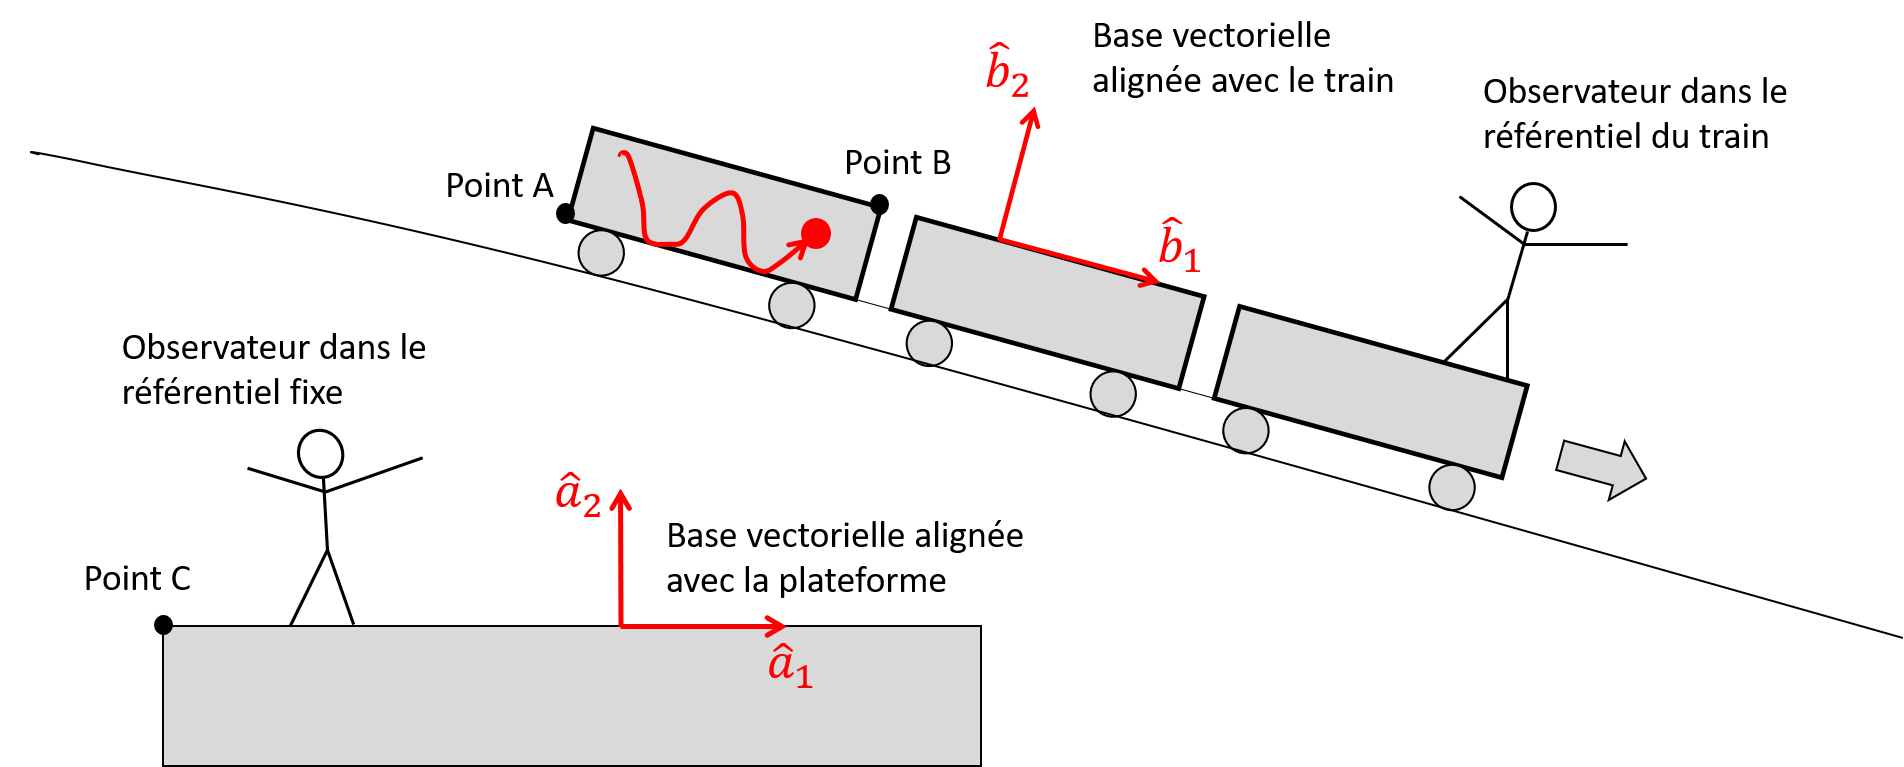
\includegraphics[width=0.90\textwidth]{train.png}
	\caption{Exemple de référentiels, points d'origine et bases vectorielles}
	\label{fig:train}
\end{figure}
%%%%%%%%%%%%%%%%%%%%%%%%%%%%%%%%%%%%%%%%%%%%%%%%%%%%%%%%%%%%%%%%%%%%%%%%%%%%%%%

La figure \ref{fig:train} illustre ces concepts par un exemple où un train descend une pente à vitesse constante et un ballon rebondit sur le sol du troisième wagon. Deux bases vectorielles sont définies, une alignée avec l'horizontale et une alignée avec le train. Plusieurs points d'origine pour les mesures de position sont aussi disponibles. Finalement, deux référentiels sont définis, un référentiel attaché à la Terre (fixe) et un référentiel qui est attaché au train. Les coordonnées d'un vecteur-colonne qui décris la position du ballon:
%%%%%%%%%%%%%%%%%%%%%%%%%%%%%%%%%%%%%
\begin{equation}
\col{r}_{Ball} = \left[ \begin{array}{c} r_1 \\ r_2 \end{array} \right]
\end{equation}
%%%%%%%%%%%%%%%%%%%%%%%%%%%%%%%%%%%%%
sont illustrés pour différents choix d'origine et de base vectorielle, lorsque que le référentiel fixe est utilisé (figure \ref{fig:refex1}) et lorsque que le référentiel du train est utilisé (figure \ref{fig:refex2}). Il est à noter que les points d'origine sont ici fixés à la Terre lorsque le référentiel fixe est utilisé, et fixés au train lorsque que le référentiel du train est utilisé. Comme illustré pour cet exemple, \textbf{un changement d'origine est analogue à une translation} de la trajectoire, \textbf{un changement de base vectorielle est analogue à une rotation} de la trajectoire, et \textbf{un changement de référentiel est ici analogue à une dilatation} de la trajectoire dans la direction $\hat{b}_1$, qui correspond à la direction de la vitesse du train. 

%%%%%%%%%%%%%%%%%%%%%%%%%%%%%%%%%%%%%%%%%%%%%%%%%%%%%%%%%%%%%%%
\begin{figure}[htpb]
				%\vspace{-10pt}
        \centering
        \subfloat[Repère $\{ A, \hat{a}_1, \hat{a}_2, \hat{a}_3\}$]{
				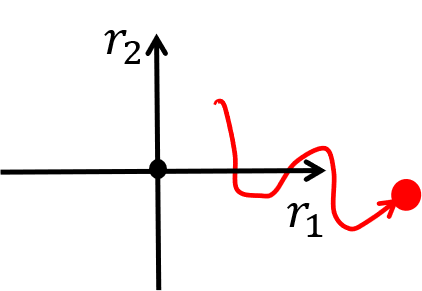
\includegraphics[width=0.23\textwidth]{ref_fixe_r_a_A.png}
				} \hspace{20pt}
				\subfloat[Repère $\{ B, \hat{a}_1, \hat{a}_2, \hat{a}_3\}$]{
				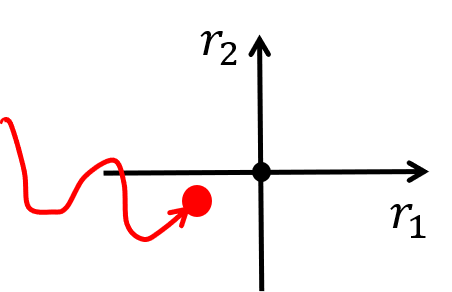
\includegraphics[width=0.24\textwidth]{ref_fixe_r_a_B.png}
				} \hspace{190pt}
				\subfloat[Repère $\{ A, \hat{b}_1, \hat{b}_2, \hat{b}_3\}$]{
				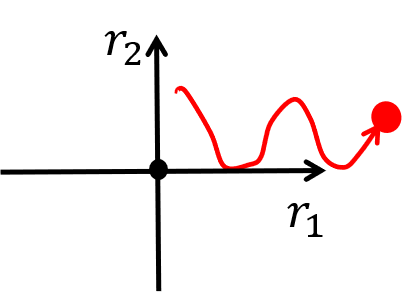
\includegraphics[width=0.22\textwidth]{ref_fixe_r_b_A.png}
				} \hspace{20pt}
				\subfloat[Repère $\{ B, \hat{b}_1, \hat{b}_2, \hat{b}_3\}$]{
				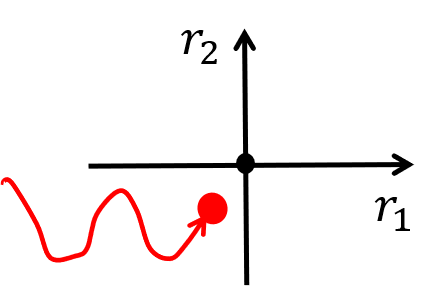
\includegraphics[width=0.24\textwidth]{ref_fixe_r_b_B.png}
				}
        \caption{Trajectoire du ballon avec un repère attaché au \textbf{référentiel fixe}}
				\label{fig:refex1}
\end{figure}
%%%%%%%%%%%%%%%%%%%%%%%%%%%%%%%%%%%%%%%%%%%%%%%%%%%%%%%%%%%%%%%%%

%%%%%%%%%%%%%%%%%%%%%%%%%%%%%%%%%%%%%%%%%%%%%%%%%%%%%%%%%%%%%%%
\begin{figure}[htpb]
				%\vspace{-10pt}
        \centering
				\subfloat[Repère $\{ A, \hat{a}_1, \hat{a}_2, \hat{a}_3\}$]{
				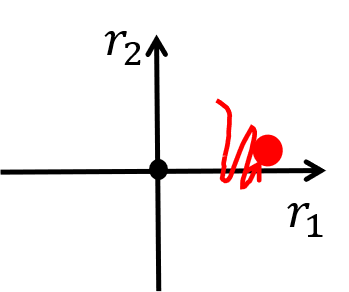
\includegraphics[width=0.22\textwidth]{ref_train_r_a_A.png}
				} \hspace{20pt}
				\subfloat[Repère $\{ B, \hat{a}_1, \hat{a}_2, \hat{a}_3\}$]{
				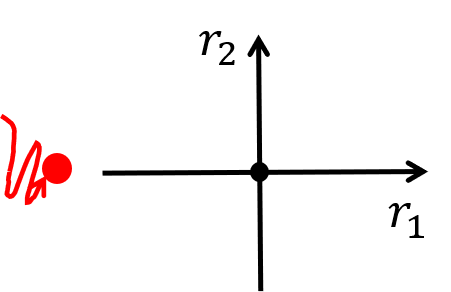
\includegraphics[width=0.25\textwidth]{ref_train_r_a_B.png}
				} \hspace{190pt}
				\subfloat[Repère $\{ A, \hat{b}_1, \hat{b}_2, \hat{b}_3\}$]{
				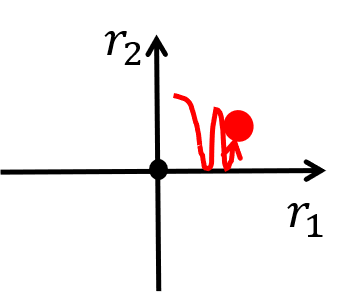
\includegraphics[width=0.22\textwidth]{ref_train_r_b_A.png}
				} \hspace{20pt}
				\subfloat[Repère $\{ B, \hat{b}_1, \hat{b}_2, \hat{b}_3\}$]{
				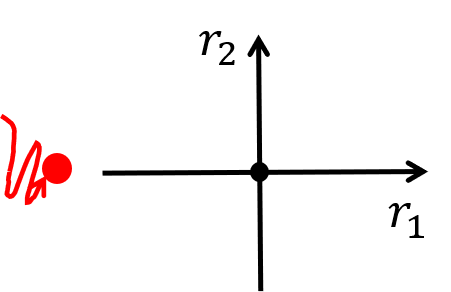
\includegraphics[width=0.25\textwidth]{ref_train_r_a_B.png}
				}
        \caption{Trajectoire du ballon avec un repère attaché au \textbf{référentiel du train}}
				\label{fig:refex2}
\end{figure}
%%%%%%%%%%%%%%%%%%%%%%%%%%%%%%%%%%%%%%%%%%%%%%%%%%%%%%%%%%%%%%%%%

